\documentclass[12pt,a4paper]{article}

\usepackage[a4paper,margin=2.4cm]{geometry}
\usepackage[T1]{fontenc}
\usepackage[utf8]{inputenc}
\usepackage{lmodern}
\usepackage{amsmath}
\usepackage{amssymb}
\usepackage{amsthm}
\usepackage{array}
\usepackage{booktabs}
\usepackage{graphicx}
\usepackage{longtable}
\usepackage{tabularx}
\usepackage{url}
\usepackage{hyperref}
\usepackage{float}

\hypersetup{
    colorlinks=true,
    linkcolor=black,
    citecolor=black,
    urlcolor=blue
}

\newtheorem{proposition}{Proposition}
\newcolumntype{Y}{>{\raggedright\arraybackslash}X}
\newcolumntype{L}[1]{>{\raggedright\arraybackslash}p{#1}}
\newcolumntype{C}[1]{>{\centering\arraybackslash}p{#1}}

\linespread{1.12}\selectfont
\setlength{\parindent}{0pt}
\setlength{\parskip}{0.12cm}

\title{\textbf{Vietnamese Handwriting OCR Under Adverse Conditions}\\
\large A shared-backbone study on clean-line accuracy, degraded-condition robustness, runtime inference, and mobile deployment}

\author{%
Nguyen Han Nhu (SE183644), Nguyen Duong Duy (SE182252),\\
Trinh Minh Khoa (SE182715), Doan Ngoc Quoc Dat (SE183236),\\
Ho Huu Huy (SE192782)\\[0.4em]
FPT University, Vietnam\\
\texttt{nhunhse183644@fpt.edu.vn, duyndse182252@fpt.edu.vn,}\\
\texttt{khoatmse182715@fpt.edu.vn, datdnqse183236@fpt.edu.vn}
}

\date{March 2026}

\begin{document}

\maketitle

\begin{abstract}
This report presents the development and evaluation of a Vietnamese handwriting OCR system under both clean and adverse imaging conditions. Rather than treating clean OCR and degraded-condition OCR as disconnected tasks, the study is organized around one shared CNN--BiLSTM--CTC backbone whose operating profiles are analyzed under different deployment constraints. The best clean offline profile, \emph{Selective Token Correction OCR}, achieves a character error rate (CER) of 0.019588, a word error rate (WER) of 0.052584, and a line-level exact-match score of 72.64\% on grouped validation data. The strongest robustness-oriented profile, \emph{Robust Bad-Condition OCR}, reduces the hard-condition CER to 0.387594 under blur, darkness, noise, and unstable capture. Under a strict one-checkpoint constraint, the most defensible final checkpoint is the blended \emph{Compromise Single-Model OCR}, which preserves a clean CER of 0.020949 while lowering the hard-condition CER to 0.470926. A runtime-oriented fixed-width profile reaches 10.34 lines per second on grouped validation data while keeping nearly the same clean accuracy as the baseline. The report also includes methodological comparison against representative OCR families such as CRNN, Tesseract, TrOCR, and PARSeq, together with qualitative examples, line-segmentation analysis, and mobile deployment evidence.
\end{abstract}

\noindent\textbf{Keywords:} Vietnamese OCR, handwriting recognition, adverse conditions, CRNN, CTC decoding, mobile OCR.

\section{Introduction}
Optical character recognition for Vietnamese handwriting remains difficult because the script contains rich diacritics, highly variable stroke shapes, inconsistent spacing, and substantial writer-to-writer variation. The problem becomes more severe when the input image is captured under blur, low illumination, compression artifacts, motion, camera shake, or naturally messy handwriting.

In practice, a deployable OCR system must satisfy several conflicting requirements at the same time. It should recognize clean white-paper handwriting accurately, remain readable in degraded conditions, support stable runtime inference, and eventually run on a mobile application. Because one model is rarely optimal for all such requirements, the research challenge is not only to improve one benchmark score, but to understand the trade-off structure of the model family.

This report follows the same experimental flow used in our slides, but it strengthens the scientific content in four ways. First, it makes the shared OCR methodology explicit. Second, it positions the project against representative OCR methods in the literature. Third, it adds formulas, diagrams, charts, and qualitative evidence. Fourth, it clarifies the final deployment recommendation under a one-checkpoint constraint.

\section{Related Work}
Modern OCR systems can be grouped into several broad families. CRNN-style recognizers combine convolutional feature extraction, recurrent sequence modeling, and CTC decoding \cite{crnn}. Tesseract is a classical OCR engine that remains historically important, but it is less suitable for unconstrained degraded Vietnamese handwriting \cite{tesseract}. More recent transformer-based methods such as TrOCR and PARSeq provide stronger global sequence modeling, but their deployment cost is significantly higher than that of a compact CRNN-style pipeline \cite{trocr,parseq}. For Vietnamese OCR, benchmark and survey work emphasizes the difficulty of diacritics, sparse public resources, and the gap between clean document OCR and unconstrained handwriting \cite{uit-hwdb,vietnamese-survey}.

\begin{table}[H]
\centering
\footnotesize
\begin{tabularx}{\textwidth}{@{}L{1.9cm}L{2.6cm}Y Y L{1.8cm}@{}}
\toprule
\textbf{Family} & \textbf{Representative work} & \textbf{Core idea} & \textbf{Relation to this project} & \textbf{Deployment fit} \\
\midrule
CRNN & Shi et al. \cite{crnn} & CNN encoder + BiLSTM + CTC transcription & Direct methodological ancestor of the backbone used in our notebooks. & High \\
Tesseract & Smith \cite{tesseract} & Classical OCR engine with adaptive recognition and document heuristics & Useful historical baseline family, but weaker for degraded Vietnamese handwriting lines. & Medium \\
TrOCR & Li et al. \cite{trocr} & Vision transformer encoder + autoregressive decoder & Strong modern OCR family, but heavier than our deployment-oriented path. & Low \\
PARSeq & Bautista and Atienza \cite{parseq} & Permuted autoregressive transformer decoding & Modern sequence-recognition reference family. & Medium \\
Vietnamese OCR context & UIT-HWDB and later surveys \cite{uit-hwdb,vietnamese-survey} & Vietnamese-specific handwriting and document-analysis benchmarking & Relevant local context, though not an identical protocol to our dataset. & Reference only \\
\bottomrule
\end{tabularx}
\caption{Methodological comparison against representative OCR families and Vietnamese OCR references.}
\label{tab:related-work}
\end{table}

The comparison in Table~\ref{tab:related-work} is methodological rather than a strict leaderboard because the datasets and protocols are different. Nevertheless, it shows why a CRNN-style backbone remains a technically reasonable choice when variable-width line OCR, ONNX export, and mobile deployment are all relevant.

\section{Dataset and Problem Setting}
The core dataset consists of Vietnamese handwritten text images already cropped at the line level. A quick inspection of the first ten samples shows that the data is dominated by long horizontal strips of handwritten text on white background, mostly addresses and short Vietnamese sentences with full diacritics. The full dataset contains 15{,}267 labeled samples. The grouped split used in the experiments contains 13{,}944 training samples and 1{,}323 grouped validation samples.

This dataset structure strongly favors line-level OCR. Consequently, the strongest results naturally appear at the character, word, line, and sentence levels. Page-level and paragraph-level OCR remain harder because they require a line-segmentation stage that is not directly supervised by the training set.

\begin{figure}[H]
\centering
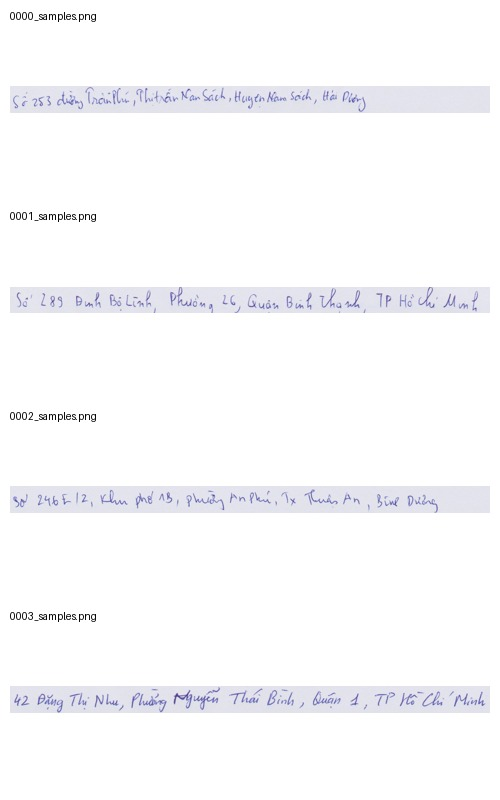
\includegraphics[width=0.82\textwidth]{fig_dataset_preview_top4.jpg}
\caption{Examples of Vietnamese handwritten line images from the dataset. The corpus is dominated by white-background line strips, which explains the strong line-level OCR performance.}
\label{fig:dataset-top4}
\end{figure}

\begin{figure}[H]
\centering
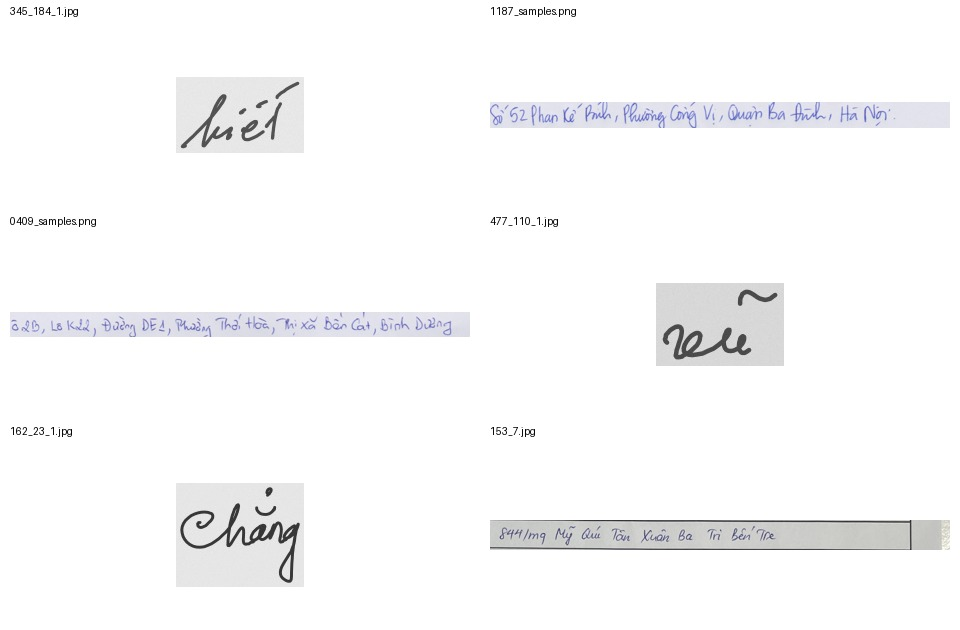
\includegraphics[width=0.85\textwidth]{fig_dataset_preview_random6.jpg}
\caption{Additional dataset samples showing variation in writing style, token length, stroke thickness, and diacritic placement.}
\label{fig:dataset-random6}
\end{figure}

\section{Methodology}
\subsection{Base recognition model}
All major systems in this project share the same OCR backbone family. Each handwritten line is converted to grayscale, normalized to a fixed height of 96 pixels, background-normalized, contrast-enhanced, and binarized before being fed into the recognizer. The recognizer itself is a CNN--BiLSTM--CTC architecture:
\begin{enumerate}
    \item five convolutional stages with channel widths 64, 128, 256, 256, and 512;
    \item a sequence reshape operation along the horizontal axis;
    \item two bidirectional LSTM layers with 256 hidden units per direction;
    \item a dense output layer over 221 target symbols;
    \item greedy CTC decoding at inference time.
\end{enumerate}

\begin{figure}[H]
\centering
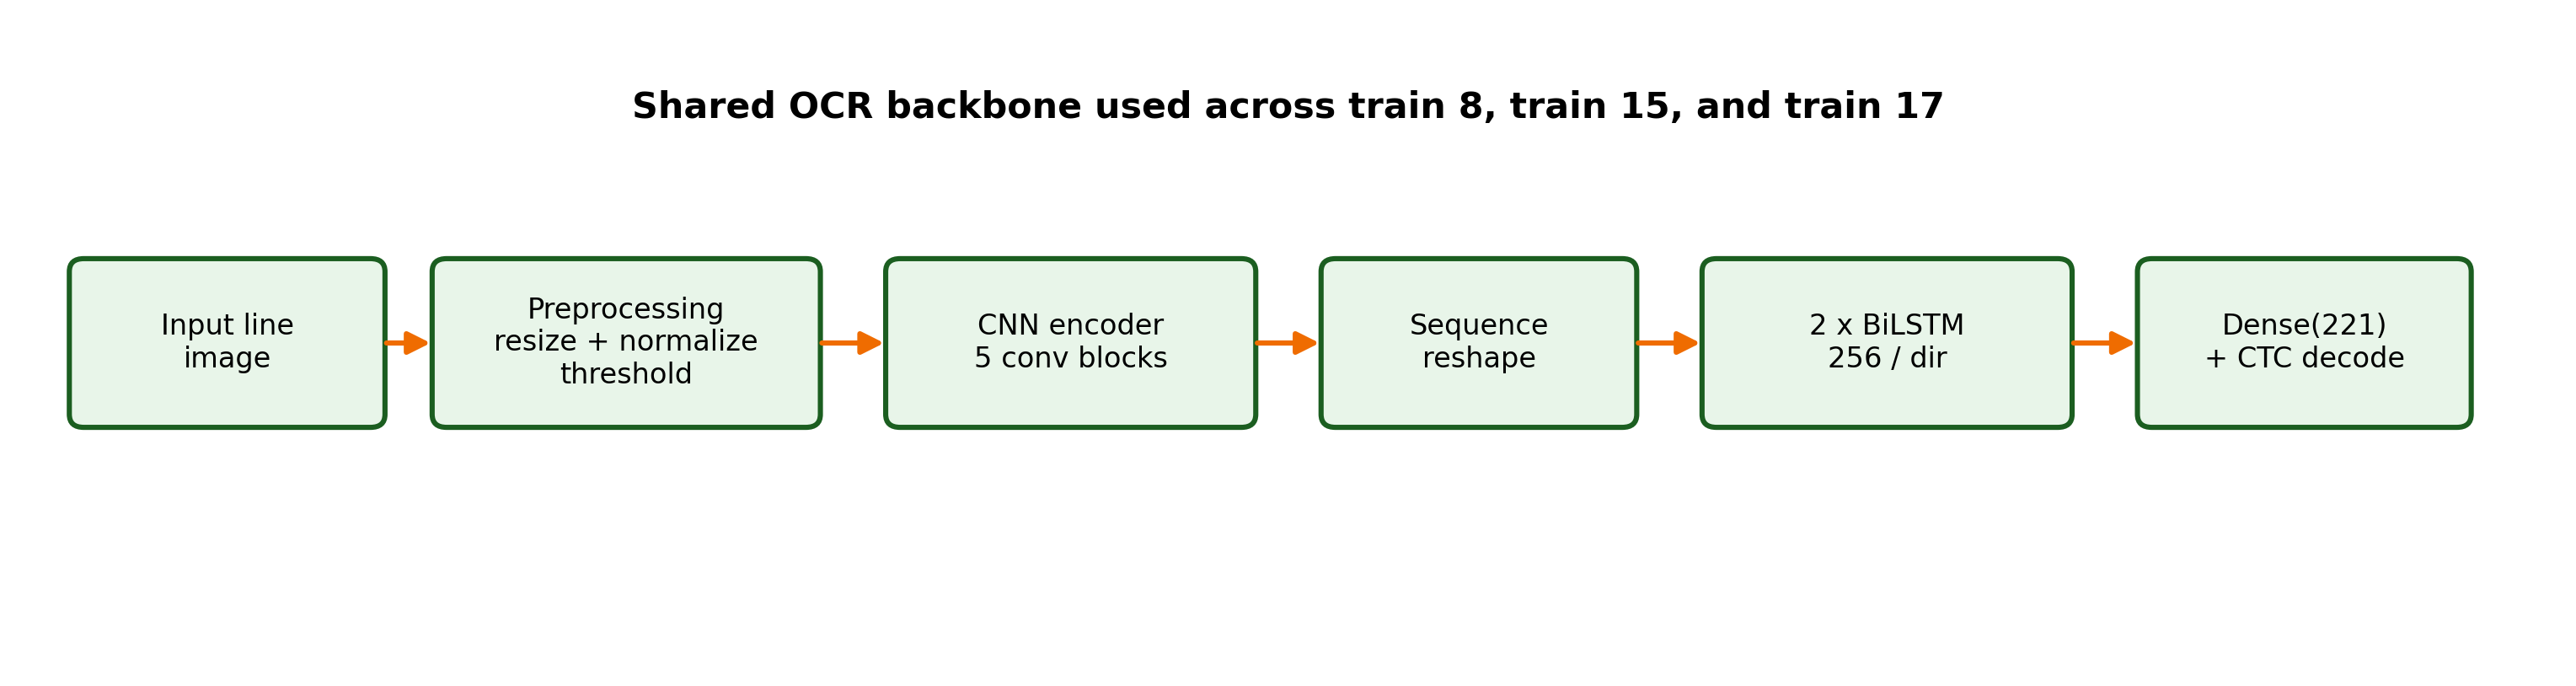
\includegraphics[width=0.98\textwidth]{fig_architecture_pipeline.png}
\caption{Shared OCR backbone used across the clean, robust, and runtime notebooks. The same CNN--BiLSTM--CTC family is reused; only the profile objective and deployment policy change.}
\label{fig:architecture}
\end{figure}

\begin{table}[H]
\centering
\small
\begin{tabular}{|l|c|c|}
\hline
\textbf{Component} & \textbf{Main setting} & \textbf{Role} \\
\hline
Input normalization & height = 96 & Standardize the line image scale \\
CNN encoder & 5 conv blocks & Extract local stroke features \\
Sequence reshape & width-wise & Convert feature map to temporal sequence \\
BiLSTM stack & 2 layers, 256/dir & Model left-to-right and right-to-left context \\
Output layer & Dense(221) & Symbol probabilities per time step \\
Decoder & Greedy CTC & Convert framewise logits to text sequence \\
\hline
\end{tabular}
\caption{Backbone structure shared by the major OCR configurations in this project.}
\label{tab:backbone}
\end{table}

\subsection{Token-level correction}
Once the OCR backbone became difficult to improve on clean white-paper lines, a token-level correction stage was explored. The key idea is to correct small token mistakes, such as missing Vietnamese diacritics or near-character substitutions, without rewriting an entire sentence. This stage operates conservatively: digits must be preserved, punctuation changes are restricted, and only a small number of token edits may be accepted.

This design explains why the clean offline gain is real but modest. The correction layer primarily serves as a precision enhancer for already strong line-level OCR. It is useful for offline evaluation, but it is not automatically the right choice for runtime deployment.

\subsection{Method of the best clean-paper profile}
The strongest clean-paper configuration in this study is the profile referred to in the experiments as \emph{Selective Token Correction OCR}. It combines the shared backbone with a fixed inference width of 2304 and a highly selective token-correction layer. The fixed-width recognizer provides stable line decoding, while the second stage repairs only a few suspicious tokens when the sentence-level score improves and the structural constraints are preserved.

This is why the clean profile reaches the best line-level offline result: CER 0.019588, WER 0.052584, and exact-match 72.64\% on grouped validation data.

\subsection{Method of the best bad-condition profile}
The strongest bad-condition configuration keeps the same shared OCR backbone, but changes the selection objective. Instead of favoring the highest clean exact-match score, it emphasizes robustness under blur, darkness, noise, compression artifacts, perspective shifts, and unstable capture. This profile is reported as \emph{Robust Bad-Condition OCR}.

Its importance is conceptual as well as practical. It shows that adverse-condition robustness is not just a matter of turning on stronger preprocessing. It requires a profile whose objective is robustness-oriented rather than clean-paper exact-match-oriented.

\subsection{Page-to-paragraph prototype and segmentation}
To explore paragraph OCR, a prototype page pipeline was built on top of the line recognizer. The page image is first cropped to the white-paper region, then lightly deskewed, thresholded, processed with connected components, and segmented into candidate line boxes. These boxes are merged, sorted, and passed one by one to the same line recognizer. The resulting lines are then concatenated into a paragraph-level text output.

\begin{figure}[H]
\centering
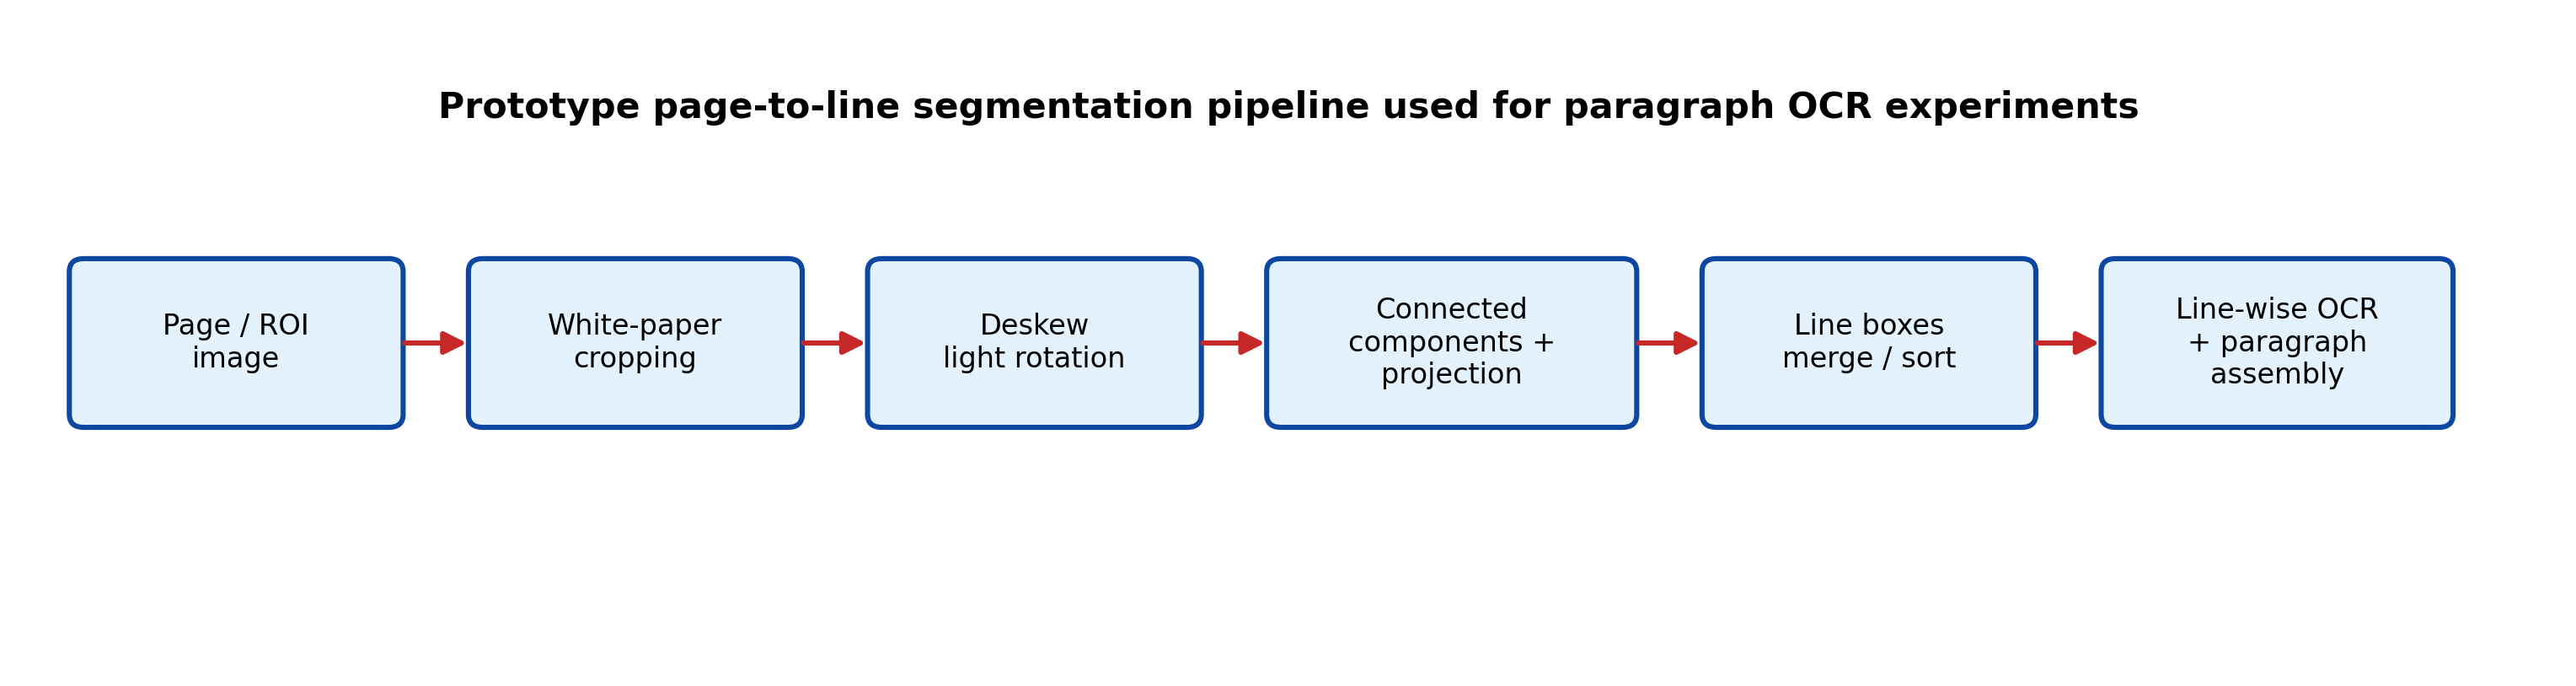
\includegraphics[width=0.98\textwidth]{fig_segmentation_pipeline.png}
\caption{Prototype page-to-line segmentation pipeline. This component enables paragraph OCR experiments, but it remains much weaker than the line recognizer itself.}
\label{fig:segmentation}
\end{figure}

The segmentation mechanism is useful as a research extension, but it remains error-prone because the training data is not page-based. Over-segmentation, fragmented lines, and incorrect ordering remain the dominant failure modes.

\section{Experimental Setup}
The experiments are evaluated using character error rate (CER), word error rate (WER), and exact-match accuracy at the line level. Runtime behavior is measured through batch throughput and per-line latency on GPU evaluation. Let $\hat{y}_i$ be the predicted text and $y_i$ the ground truth text of sample $i$. The main metrics are:
\begin{align}
\mathrm{CER} &= \frac{\sum_i \mathrm{EditDistance}_{char}(\hat{y}_i, y_i)}{\sum_i |y_i|}, \\
\mathrm{WER} &= \frac{\sum_i \mathrm{EditDistance}_{word}(\hat{y}_i, y_i)}{\sum_i |y_i|_{word}}, \\
\mathrm{ExactMatch} &= \frac{1}{N} \sum_{i=1}^{N} \mathbf{1}[\hat{y}_i = y_i].
\end{align}

For the one-checkpoint setting explored in the profile-export family, the blended profile can be written abstractly as
\begin{equation}
W_{\alpha} = (1-\alpha)W_{\text{clean}} + \alpha W_{\text{robust}},
\end{equation}
where $W_{\text{clean}}$ and $W_{\text{robust}}$ are the clean and robust weights, and $\alpha \in \{0.20, 0.35, 0.50\}$ in the evaluated blend candidates.

To formalize checkpoint selection under a one-model constraint, the trade-off objective can be written as
\begin{equation}
J_{\lambda}(m) = \lambda \cdot \mathrm{CER}_{hard}(m) + (1-\lambda)\cdot \left(1-\mathrm{ExactMatch}_{clean}(m)\right),
\end{equation}
where $m$ is a candidate profile and $\lambda \in [0,1]$ controls the importance of hard-condition robustness.

\begin{proposition}
Among the evaluated blend candidates in the shared train-8 profile-export family, the profile with $\alpha = 0.35$ is a Pareto-undominated compromise under the one-checkpoint constraint, because it reduces hard-condition CER substantially relative to the clean profile while preserving much more clean exact-match accuracy than the fully robust profile.
\end{proposition}

The degraded-condition benchmark in this project is a hard synthetic benchmark rather than a large field-collected mobile dataset. It is built from blur, noise, brightness shifts, compression artifacts, perspective distortion, and local occlusion. Therefore, the hard-condition results should be interpreted as robustness-oriented evidence rather than full field validation.

\section{Results}
\subsection{Best configurations by target condition}
Table~\ref{tab:main-results} summarizes the most relevant OCR configurations used in the final analysis. The important observation is that all of them come from the same backbone family, but their operating objectives differ.

\begin{table}[H]
\centering
\footnotesize
\begin{tabularx}{\textwidth}{|L{3.0cm}|Y|C{1.45cm}|C{1.45cm}|C{1.75cm}|C{1.45cm}|C{1.75cm}|}
\hline
\textbf{Configuration} & \textbf{Primary objective} & \textbf{Clean CER} & \textbf{Clean WER} & \textbf{Clean exact (\%)} & \textbf{Hard CER} & \textbf{Hard exact (\%)} \\
\hline
Clean Baseline OCR & Strongest line-level OCR on clean white-paper inputs & 0.019918 & 0.053734 & 72.56 & 0.562548 & 11.33 \\
Selective Token Correction OCR & Improve clean offline recognition with conservative post-correction & 0.019588 & 0.052584 & 72.64 & 0.557602 & 12.89 \\
Robust Bad-Condition OCR & Maximize degraded-condition robustness under blur, darkness, and noise & 0.028007 & 0.076146 & 63.87 & 0.387594 & 11.72 \\
Compromise Single-Model OCR & One-checkpoint trade-off between clean quality and adverse-condition robustness & 0.020949 & 0.056665 & 70.29 & 0.470926 & 11.72 \\
\hline
\end{tabularx}
\caption{Comparison of the main OCR operating profiles derived from the shared backbone family.}
\label{tab:main-results}
\end{table}

The clean best and the robust best are not the same system. This is the central empirical finding of the project. However, under a one-checkpoint deployment requirement, the \emph{Compromise Single-Model OCR} becomes the most defensible final choice.

\begin{figure}[H]
\centering
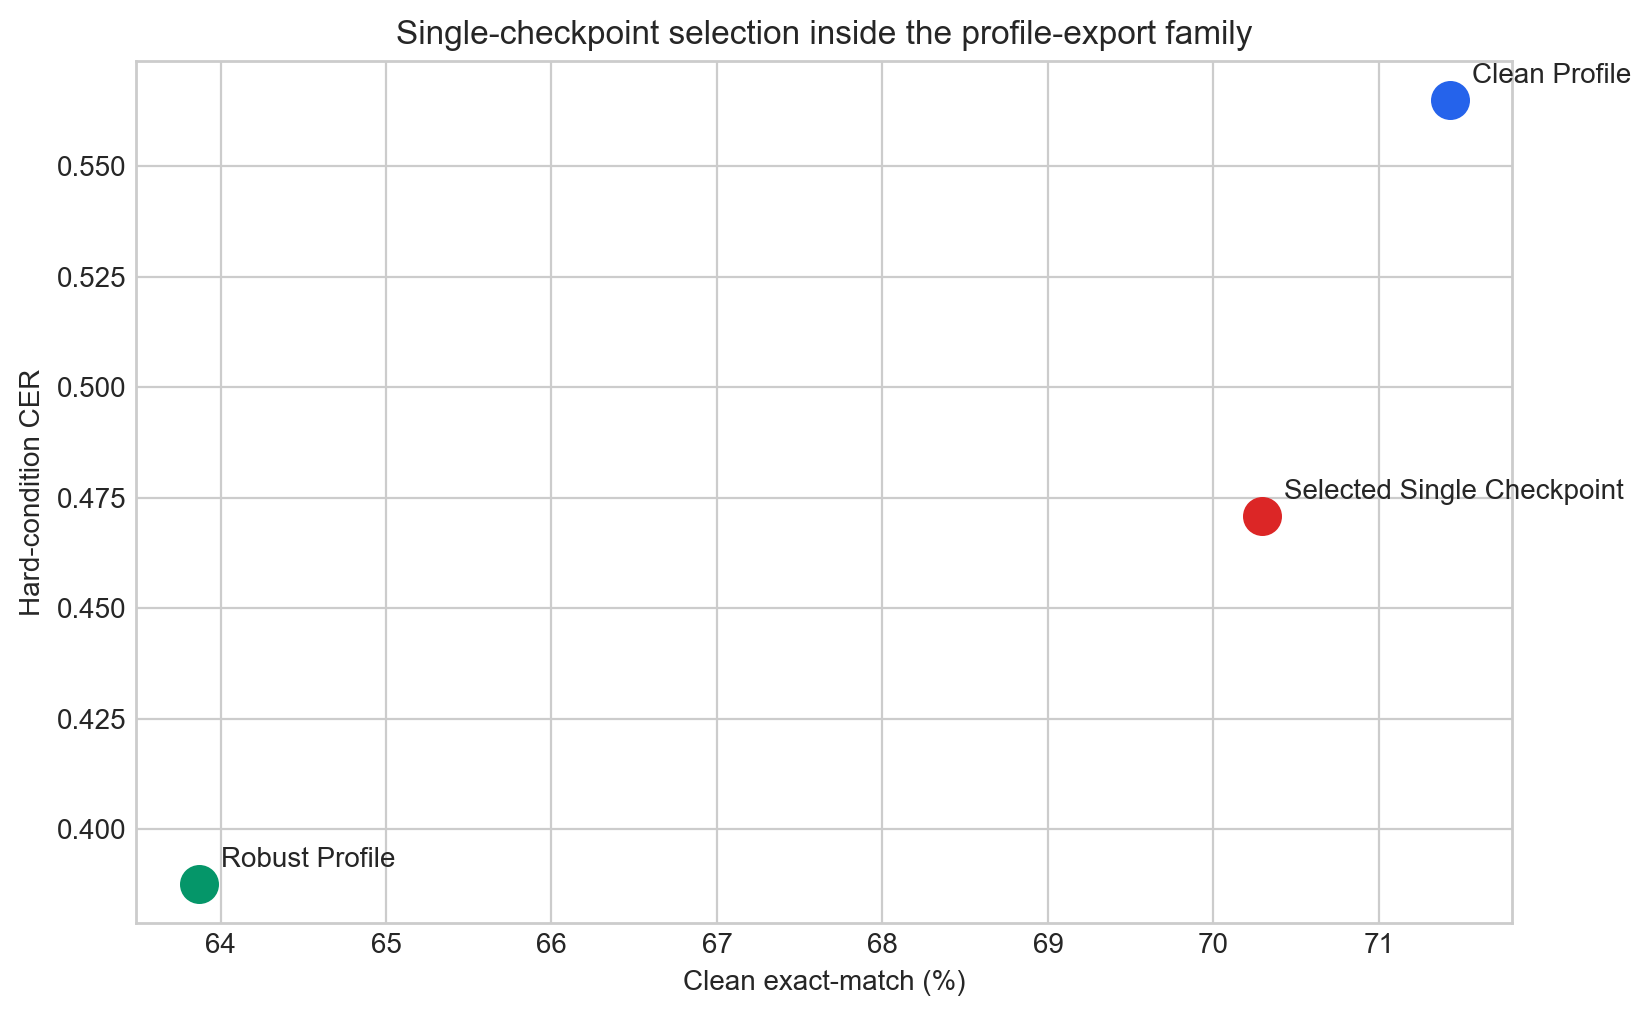
\includegraphics[width=0.84\textwidth]{fig_single_checkpoint_family_tradeoff.png}
\caption{Trade-off inside the profile-export family. The blended single-model checkpoint sits between the clean profile and the robust profile.}
\label{fig:tradeoff-family}
\end{figure}

\begin{figure}[H]
\centering
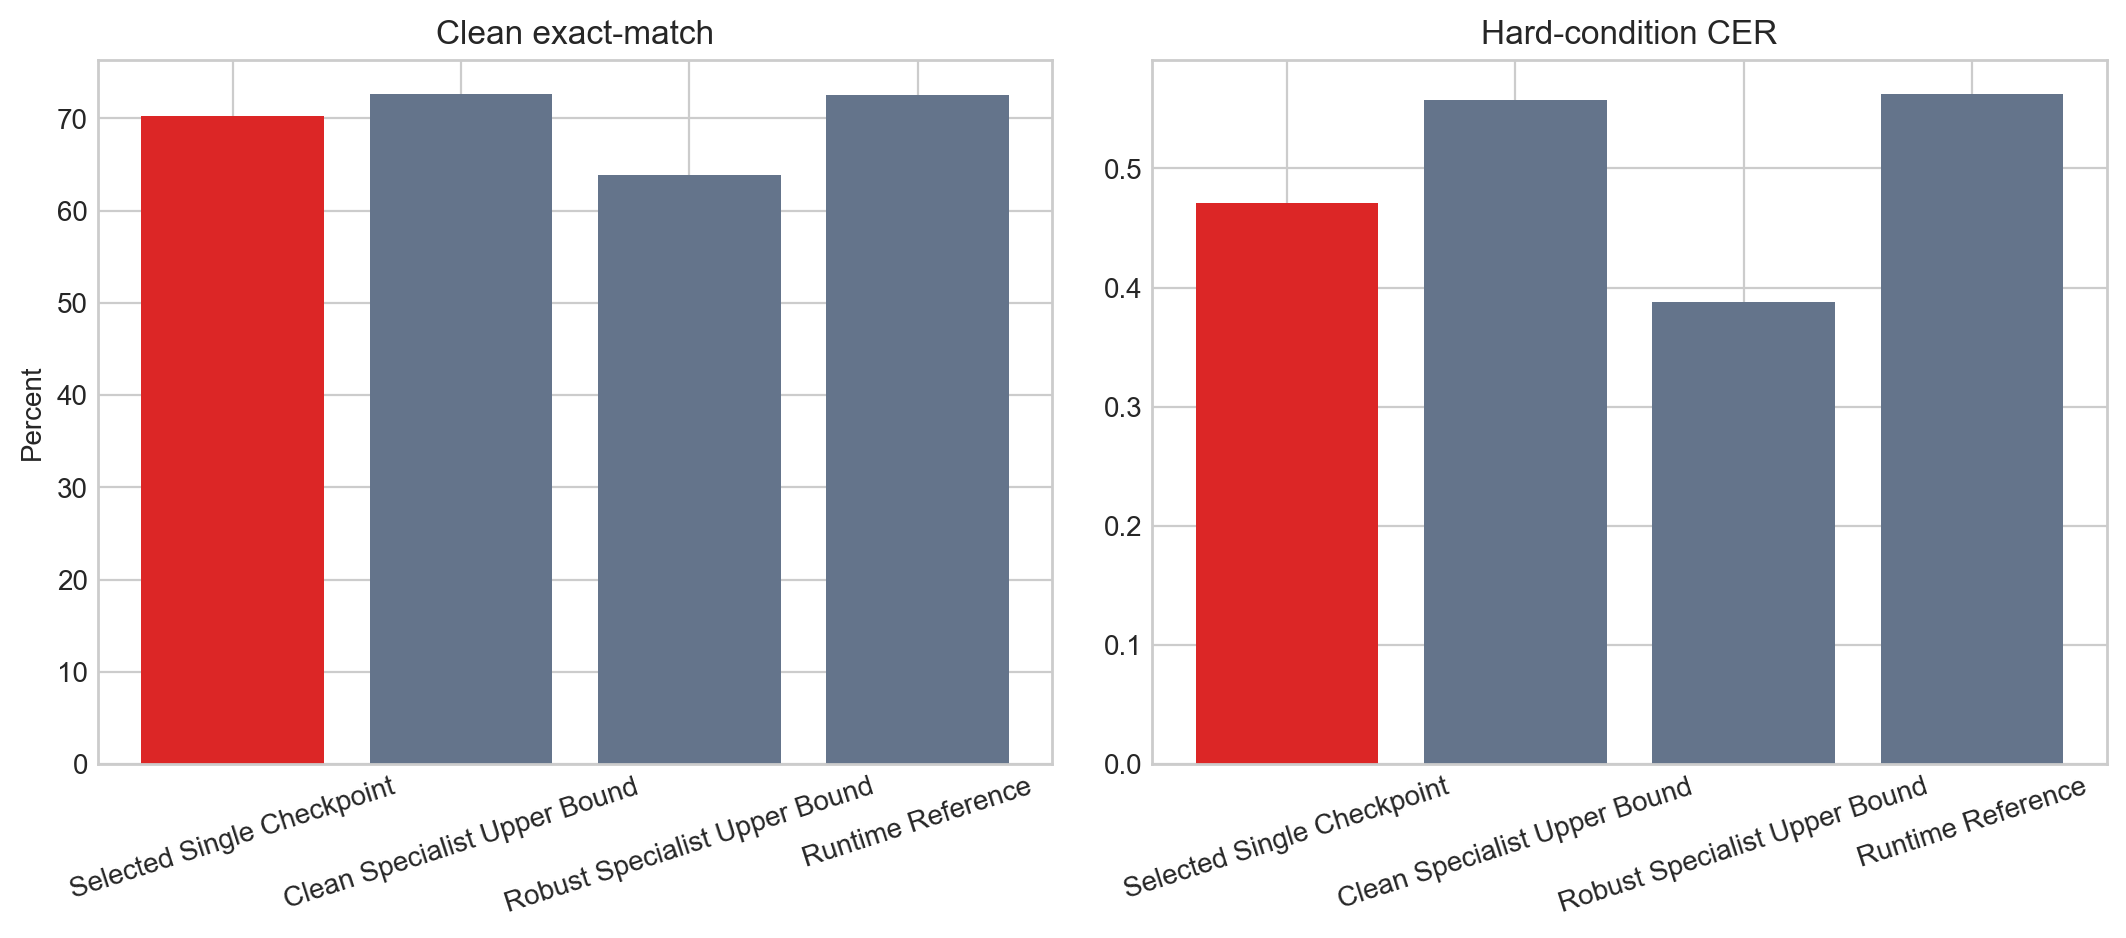
\includegraphics[width=0.92\textwidth]{fig_single_checkpoint_vs_ablations.png}
\caption{Comparison against clean-specialist, robust-specialist, and runtime-reference ablations. The single-checkpoint compromise is not the best at either extreme, but it is the most balanced one-model option.}
\label{fig:ablations}
\end{figure}

\subsection{Output-level interpretation}
At the character level, the strongest clean configuration reaches approximately 98.04\% character accuracy, while the robustness-oriented profile reaches approximately 61.24\% character accuracy under the degraded benchmark. At the word level, the clean best profile yields a WER of 5.26\%, whereas the robustness-oriented profile yields a hard-condition WER of 60.72\%.

At the line/sentence level, the best clean offline exact-match score is 72.64\%. Under adverse conditions, the exact-match score remains low for all models, but the robust profile still yields a much lower CER, meaning its outputs are materially closer to the target text even when exact string equality is difficult.

\begin{figure}[H]
\centering
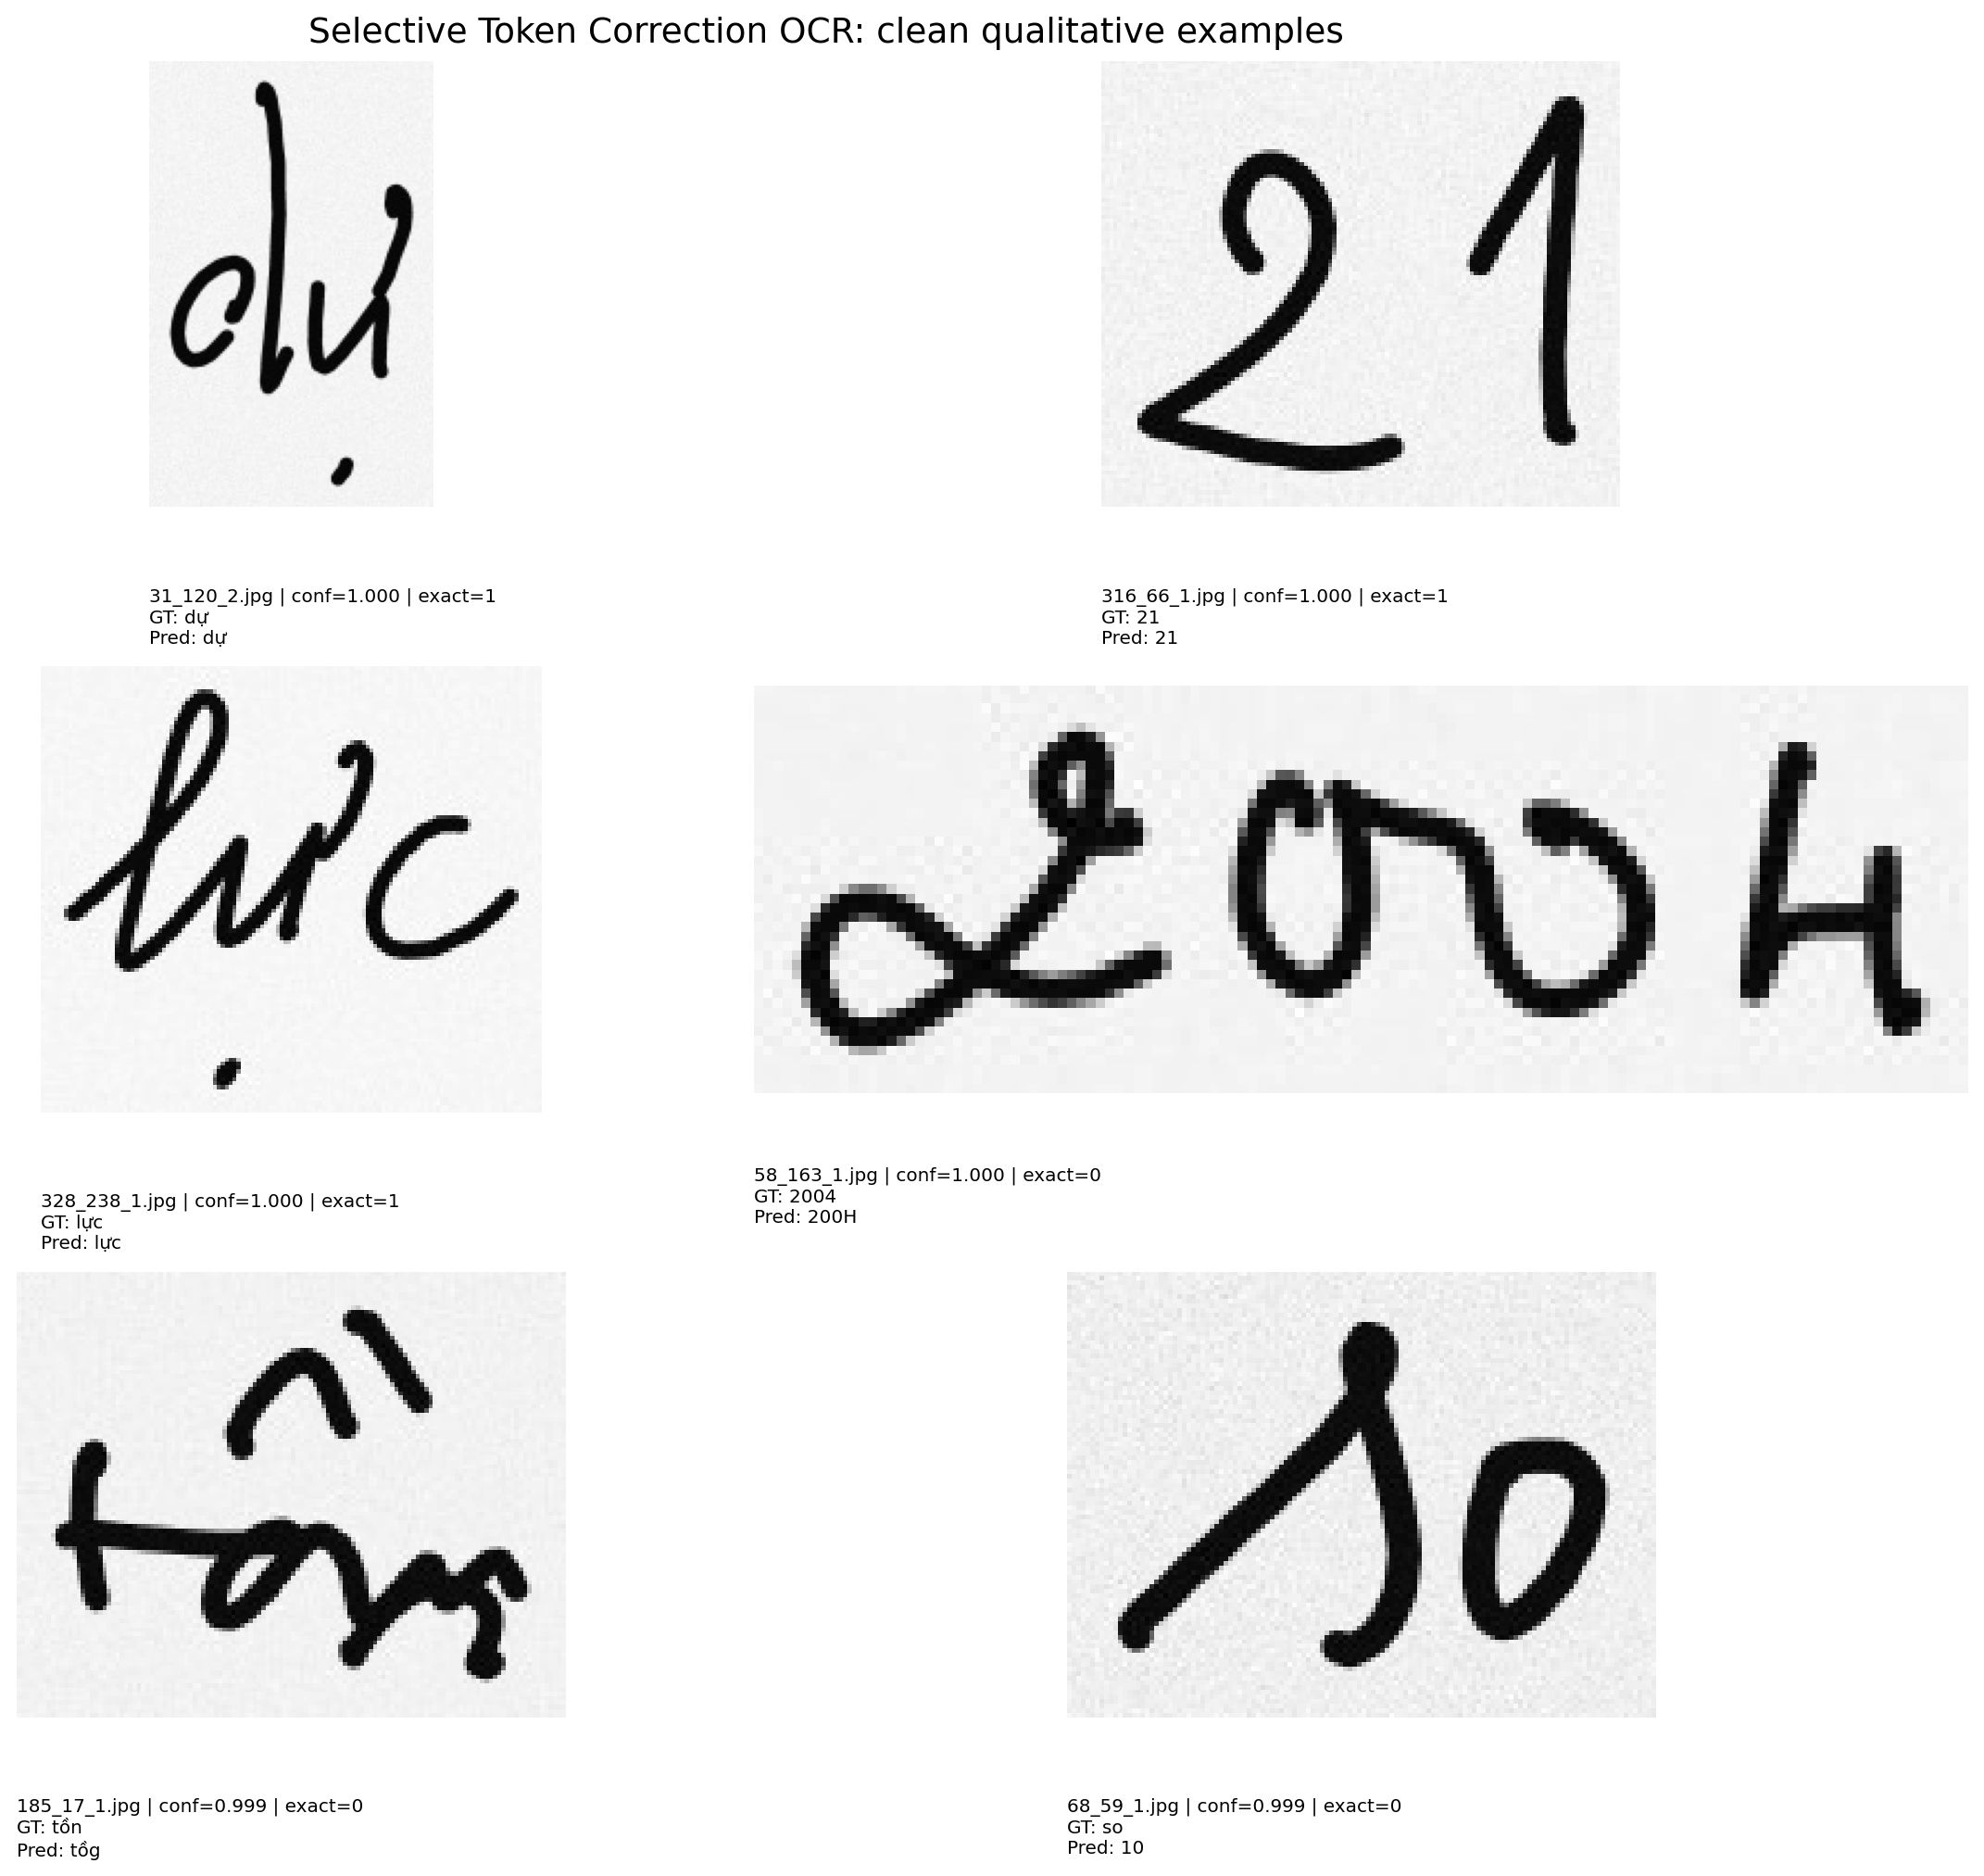
\includegraphics[width=0.92\textwidth]{fig_qualitative_clean_examples.png}
\caption{Qualitative clean-condition examples. The system is strongest on stable white-background lines with good stroke contrast and full Vietnamese diacritics.}
\label{fig:qual-clean}
\end{figure}

\begin{figure}[H]
\centering
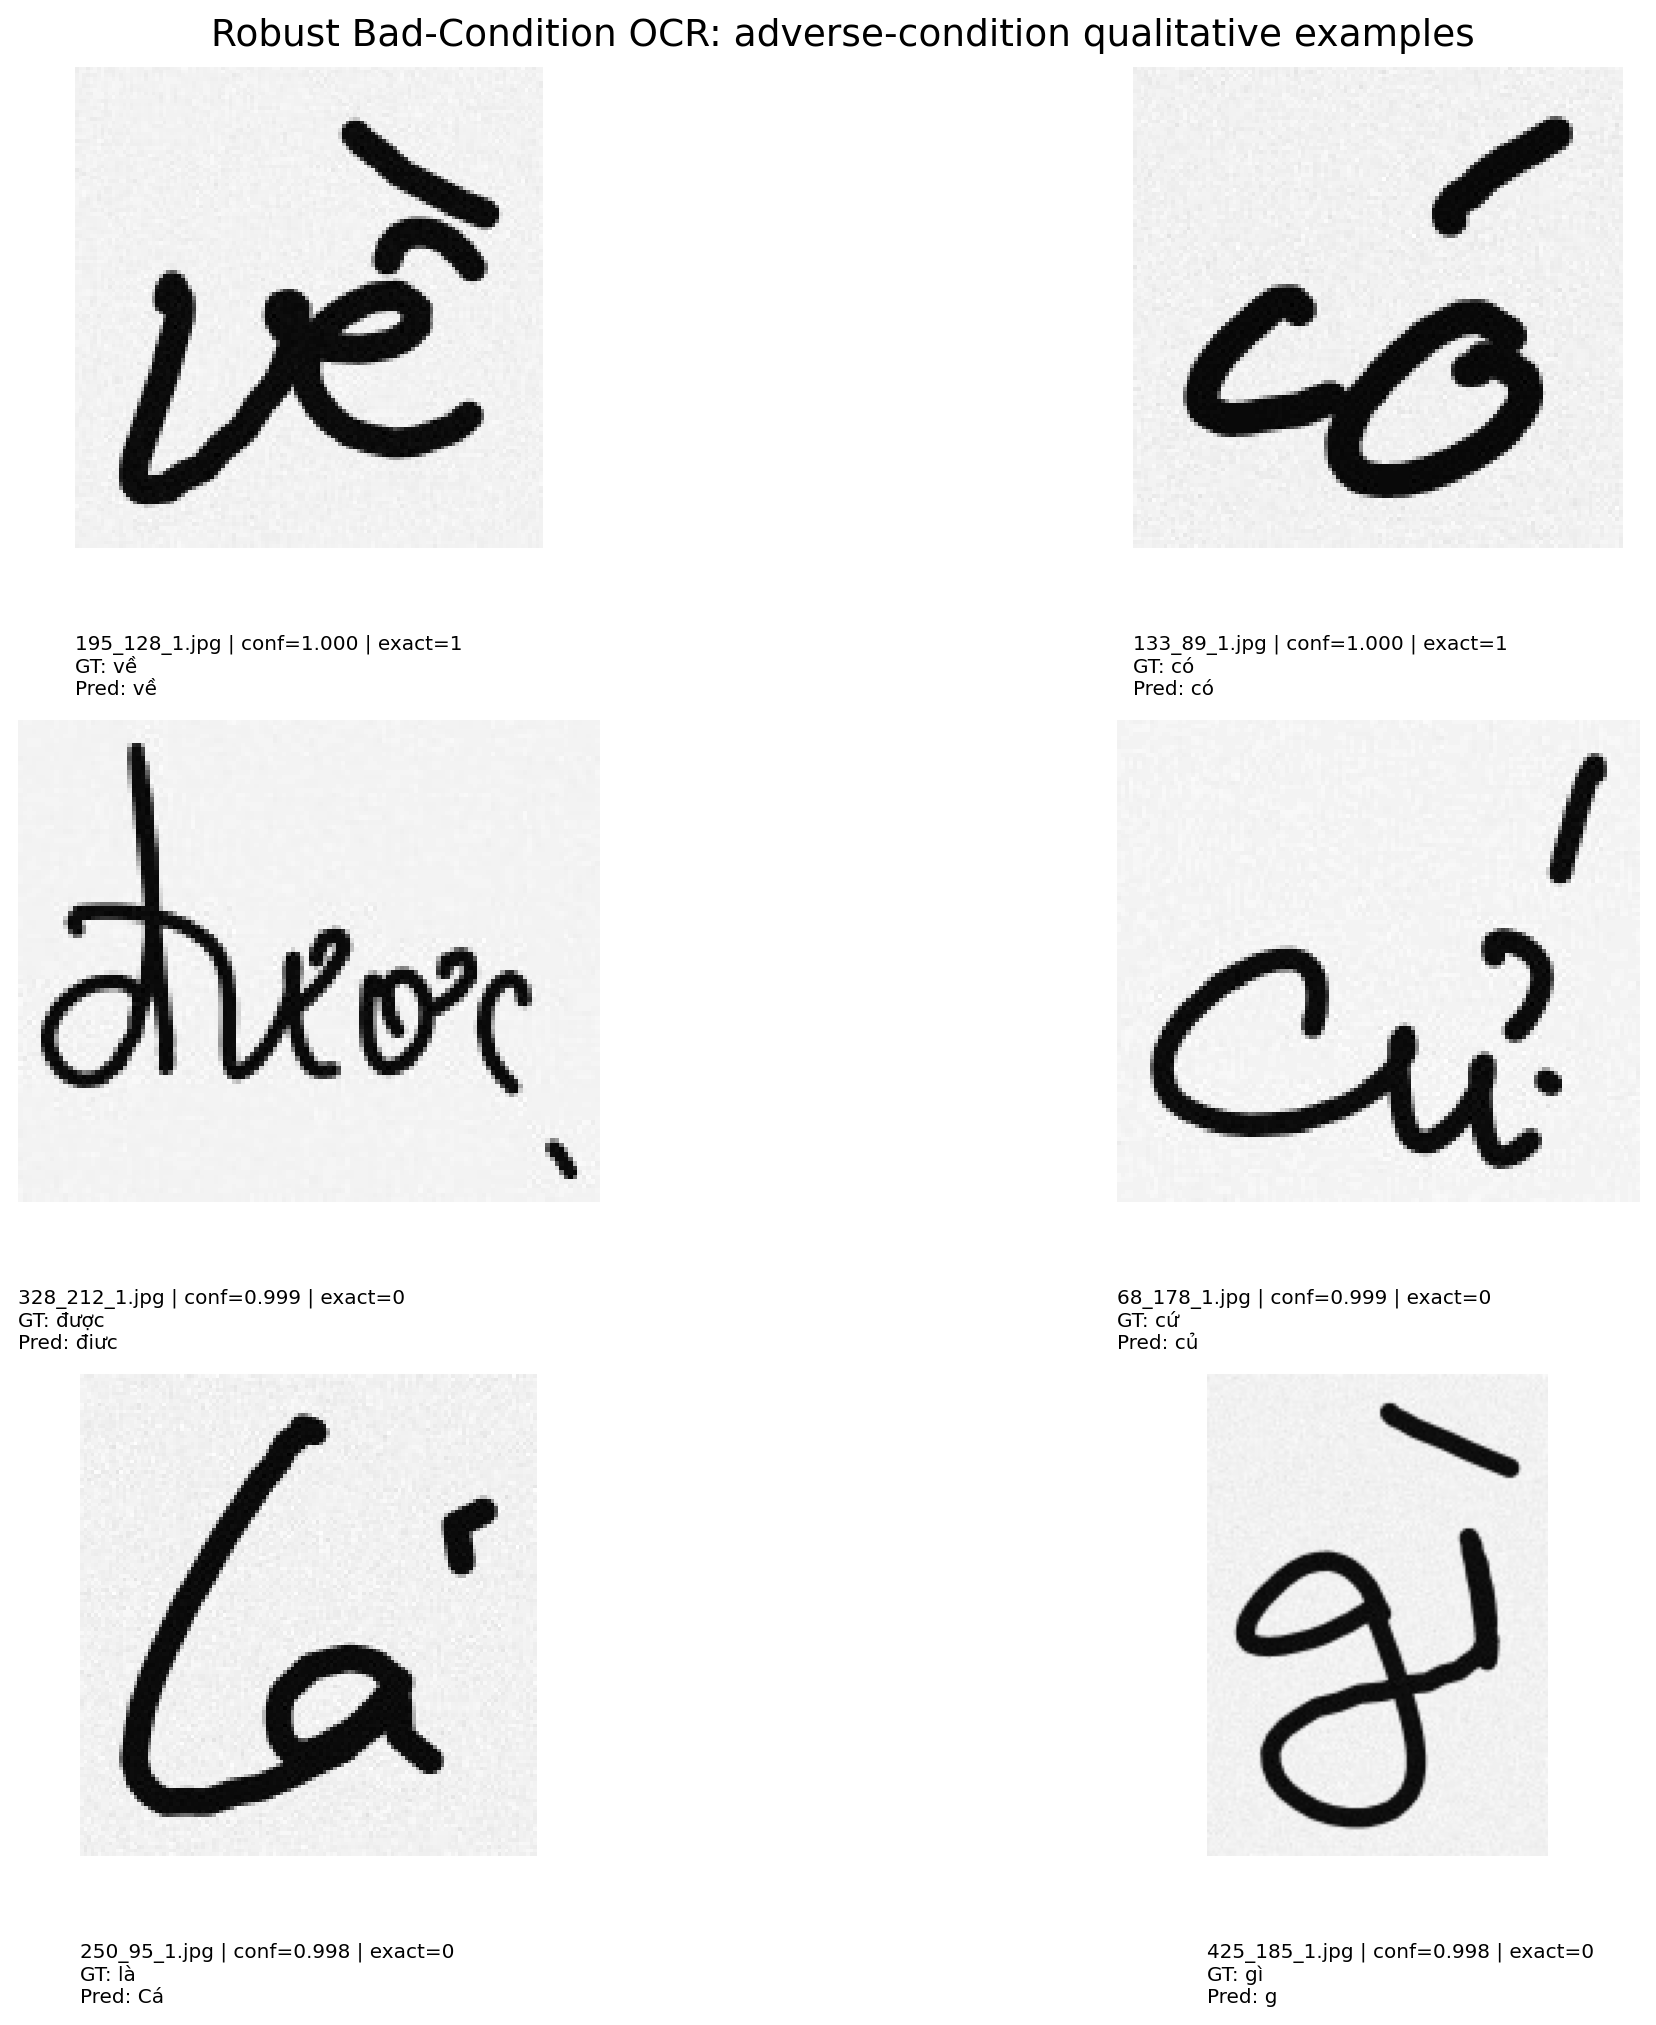
\includegraphics[width=0.92\textwidth]{fig_qualitative_hard_examples.png}
\caption{Qualitative hard-condition examples. Typical failure sources include blur, weak contrast, stroke overlap, and unstable or missing diacritics.}
\label{fig:qual-hard}
\end{figure}

\subsection{Runtime evaluation}
Table~\ref{tab:runtime-results} compares the two runtime-oriented policies on the clean grouped validation set.

\begin{table}[H]
\centering
\footnotesize
\begin{tabularx}{\textwidth}{|L{4.8cm}|C{1.45cm}|C{1.45cm}|C{1.55cm}|C{2.55cm}|C{2.55cm}|}
\hline
\textbf{Runtime profile} & \textbf{CER} & \textbf{WER} & \textbf{Exact (\%)} & \textbf{Batch throughput (lines/s)} & \textbf{Single-line latency (ms)} \\
\hline
Realtime Runtime OCR (quality\_2304 profile) & 0.019918 & 0.053734 & 72.56 & 10.34 & 505.93 \\
Adaptive Runtime OCR & 0.020071 & 0.055214 & 72.34 & 9.44 & 473.19 \\
\hline
\end{tabularx}
\caption{Runtime-oriented comparison on grouped validation data.}
\label{tab:runtime-results}
\end{table}

Although the adaptive policy slightly reduces the average single-sample latency, it degrades both recognition quality and batch throughput. Therefore, the selected runtime setting is the fixed-width quality\_2304 profile rather than the adaptive profile.

\subsection{Page-to-paragraph OCR}
The page-level prototype remains weak. The best page demo result yields a CER of 1.133593 and an exact page-level match of only 16.67\%. This confirms that the project should not claim paragraph OCR as a finished capability.

\begin{figure}[H]
\centering
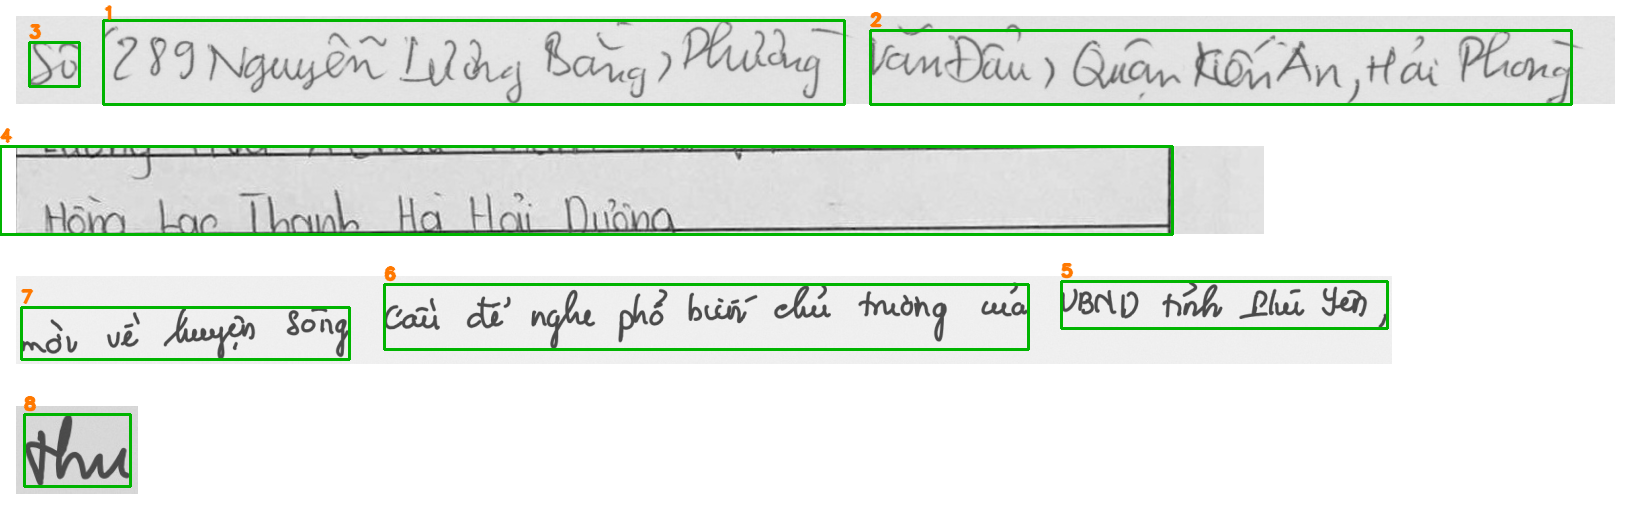
\includegraphics[width=\textwidth]{fig_page_overlay_quality2304.png}
\caption{Prototype page-level segmentation and OCR overlay. Over-segmentation and line fragmentation remain the main bottlenecks of paragraph OCR.}
\label{fig:page-overlay}
\end{figure}

\begin{figure}[H]
\centering
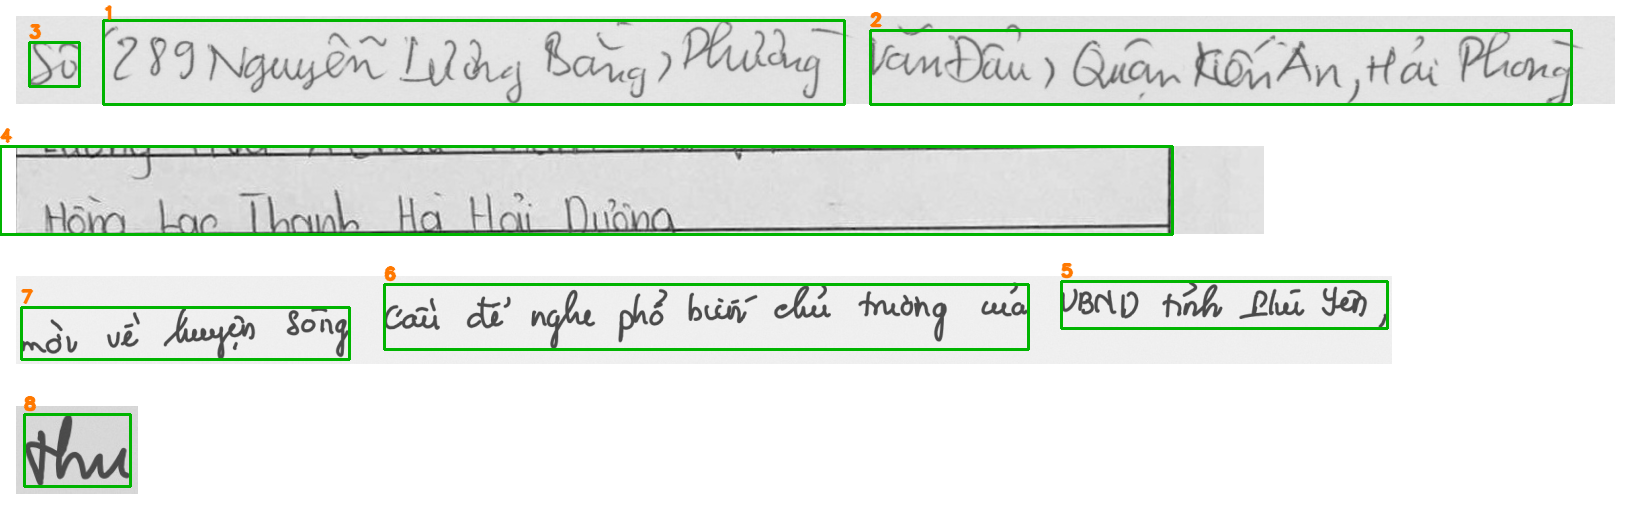
\includegraphics[width=0.95\textwidth]{fig_page_pipeline_failure.png}
\caption{Representative page-level failure case generated from the runtime notebook. The line recognizer is strong, but the segmentation stage still fragments or merges text incorrectly.}
\label{fig:page-failure}
\end{figure}

\section{Discussion}
The experiments support one coherent research direction: a shared OCR backbone evaluated through multiple operating profiles. This framing is stronger than treating clean OCR and bad-condition OCR as unrelated subprojects. The clean specialist, robust specialist, runtime profile, and one-checkpoint compromise are all derived from the same backbone family and therefore form one interpretable trade-off study.

The empirical results also explain why the final recommendation depends on the deployment constraint. If the goal is the highest clean offline accuracy, the selective token-correction profile is the best choice. If the goal is robustness under blur, darkness, and unstable capture, the robust profile is the best choice. If only one checkpoint can be deployed, the blended compromise profile is the most defensible answer because it preserves most clean accuracy while materially reducing hard-condition CER.

The methodology is also well aligned with the literature. Relative to Tesseract, the project uses a trainable sequence-recognition pipeline better suited to unconstrained handwriting. Relative to heavy transformer OCR, it stays closer to the CRNN family, which is more compatible with ONNX export, line-level inference, and mobile demonstration.

\section{Mobile Deployment Considerations}
An Android proof-of-concept application has already been prepared for live OCR demonstration. The application captures frames through CameraX, crops a central ROI, applies preprocessing, runs ONNX inference, and decodes the recognized text. This is sufficient to demonstrate the mobile direction of the project.

However, the artifact lineage must be stated precisely. The main scientific result of this report is the shared-backbone analysis and the one-checkpoint compromise recommendation. The current mobile prototype uses exported clean and robust ONNX specialist models from the same backbone family. Therefore, the APK should be interpreted as deployment evidence from the same model family rather than as the exact artifact used for the final single-checkpoint quantitative claim.

\section{Conclusion}
This study shows that Vietnamese handwriting OCR under adverse conditions is best analyzed as one shared-backbone research direction with multiple operating profiles. The strongest clean-paper profile is \emph{Selective Token Correction OCR}. The strongest degraded-condition profile is \emph{Robust Bad-Condition OCR}. The best runtime policy is the fixed-width quality\_2304 profile. Under a strict one-checkpoint constraint, the most defensible final model is \emph{Compromise Single-Model OCR}.

The project therefore reaches a coherent and scientifically defensible conclusion. Line-level OCR on clean paper is already strong, degraded-condition OCR can be improved substantially through robustness-oriented profile selection, and mobile deployment is feasible through ONNX export. At the same time, paragraph OCR and exact mobile equivalence remain open engineering tasks rather than solved claims.

\begin{thebibliography}{99}
\bibitem{crnn}
B. Shi, X. Bai, and C. Yao,
\newblock ``An End-to-End Trainable Neural Network for Image-based Sequence Recognition and Its Application to Scene Text Recognition,''
\newblock \emph{arXiv preprint arXiv:1507.05717}, 2015.
\newblock Available: \url{https://arxiv.org/abs/1507.05717}

\bibitem{tesseract}
R. Smith,
\newblock ``An Overview of the Tesseract OCR Engine,''
\newblock in \emph{Proceedings of the Ninth International Conference on Document Analysis and Recognition (ICDAR)}, 2007.
\newblock Available: \url{https://research.google/pubs/an-overview-of-the-tesseract-ocr-engine/}

\bibitem{trocr}
M. Li, T. Lv, J. Cui, L. Lu, Y. Florencio, D. Zhang, and F. Wei,
\newblock ``TrOCR: Transformer-based Optical Character Recognition with Pre-trained Models,''
\newblock \emph{arXiv preprint arXiv:2109.10282}, 2021.
\newblock Available: \url{https://arxiv.org/abs/2109.10282}

\bibitem{parseq}
D. Bautista and R. Atienza,
\newblock ``Scene Text Recognition with Permuted Autoregressive Sequence Models,''
\newblock \emph{arXiv preprint arXiv:2207.06966}, 2022.
\newblock Available: \url{https://arxiv.org/abs/2207.06966}

\bibitem{uit-hwdb}
\newblock ``UIT-HWDB: Using Transferring Method to Construct a Novel Benchmark for Evaluating Unconstrained Handwriting Image Recognition in Vietnamese,''
\newblock \emph{arXiv preprint arXiv:2211.05407}, 2022.
\newblock Available: \url{https://arxiv.org/abs/2211.05407}

\bibitem{vietnamese-survey}
\newblock ``Vietnamese Document Analysis and Recognition: A Survey and Open Challenges,''
\newblock \emph{arXiv preprint arXiv:2506.05061}, 2025.
\newblock Available: \url{https://arxiv.org/abs/2506.05061}
\end{thebibliography}

\end{document}
